\documentclass[10pt]{article}
% Shared preamble for the second-brain PDF handouts.  Compile with:  latexmk -pdf -outdir=build <file>.tex
\usepackage[T1]{fontenc}
\usepackage{lmodern}
\usepackage[a4paper,margin=18mm]{geometry}
\usepackage{amsmath,amssymb,mathtools,bm}
\usepackage{siunitx}
\sisetup{per-mode=symbol,detect-all}
\usepackage{booktabs,array,enumitem}
\usepackage{xcolor}
\usepackage{tikz}
\usetikzlibrary{arrows.meta,calc,angles,quotes,decorations.pathreplacing,positioning}
\usepackage{pgfplots}
\pgfplotsset{compat=1.18}
\usepackage[most]{tcolorbox}
\usepackage[colorlinks=true,linkcolor=blue!50!black,urlcolor=blue!50!black]{hyperref}

% palette shared with the figures (dataviz reference, light mode)
\definecolor{cBlue}{HTML}{2A78D6}
\definecolor{cOrange}{HTML}{EB6834}
\definecolor{cAqua}{HTML}{1BAF7A}
\definecolor{cViolet}{HTML}{6250D6}
\definecolor{cRed}{HTML}{E34948}
\definecolor{cInk}{HTML}{0B0B0B}
\definecolor{cMuted}{HTML}{52514E}

% boxes mirroring the Obsidian callouts
\newtcolorbox{keybox}[1][]{enhanced,colback=violet!5,colframe=cViolet,fonttitle=\bfseries,title={#1},boxrule=0.6pt,arc=2pt,left=4pt,right=4pt}
\newtcolorbox{derivbox}[1][]{enhanced,colback=black!3,colframe=cMuted,fonttitle=\bfseries,title={#1},boxrule=0.6pt,arc=2pt,left=4pt,right=4pt}
\newtcolorbox{extrabox}[1][]{enhanced,colback=blue!4,colframe=cBlue,fonttitle=\bfseries,title={Extra (beyond): #1},boxrule=0.6pt,arc=2pt,left=4pt,right=4pt}
\newtcolorbox{verifybox}[1][]{enhanced,colback=yellow!10,colframe=orange!70!black,fonttitle=\bfseries,title={Check: #1},boxrule=0.6pt,arc=2pt,left=4pt,right=4pt}

\newcommand{\dd}{\mathrm{d}}
\newcommand{\DD}{\mathrm{D}}
\newcommand{\vect}[1]{\bm{#1}}
\setlength{\parindent}{0pt}
\setlength{\parskip}{4pt}

\title{Climate, Part IV: rotating frames and the Coriolis force\\\large derivation sheet}
\author{second brain $\cdot$ chapter CL12}
\date{}
\begin{document}
\maketitle
\vspace{-2em}

\section*{1. Frames and the transformation rule}
\begin{center}
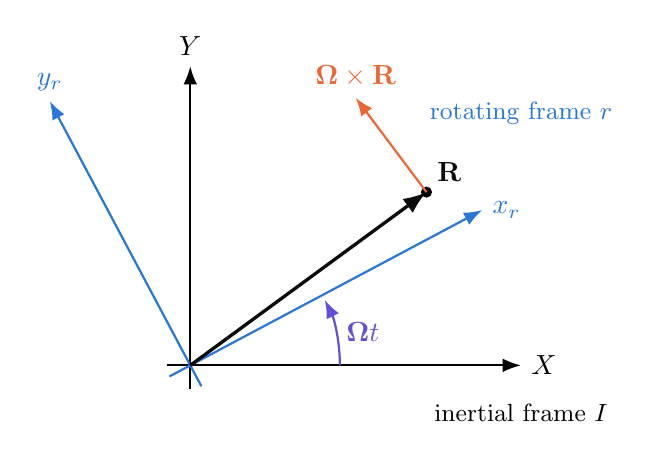
\begin{tikzpicture}[scale=1.0]
  \draw[-{Latex},thick] (-0.3,0) -- (4.2,0) node[right] {$X$};
  \draw[-{Latex},thick] (0,-0.3) -- (0,3.8) node[above] {$Y$};
  \begin{scope}[rotate=28]
    \draw[-{Latex},thick,cBlue] (-0.3,0) -- (4.2,0) node[right] {$x_r$};
    \draw[-{Latex},thick,cBlue] (0,-0.3) -- (0,3.8) node[above] {$y_r$};
  \end{scope}
  \coordinate (P) at (3.0,2.2);
  \draw[-{Latex},very thick,cInk] (0,0) -- (P) node[above right] {$\mathbf R$};
  \fill (P) circle (2pt);
  \draw[-{Latex},thick,cOrange] (P) -- ($(P)+(-0.9,1.2)$) node[above] {$\bm\Omega\times\mathbf R$};
  \draw[-{Latex},cViolet,thick] (1.9,0) arc[start angle=0,end angle=26,radius=1.9] node[midway,right] {$\bm\Omega t$};
  \node[cBlue,font=\small] at (4.2,3.2) {rotating frame $r$};
  \node[font=\small] at (4.2,-0.6) {inertial frame $I$};
\end{tikzpicture}
\end{center}

\begin{keybox}[Transformation rule: any vector $\mathbf A$]
\[
\Bigl(\frac{\dd\mathbf A}{\dd t}\Bigr)_{\!I}=\Bigl(\frac{\dd\mathbf A}{\dd t}\Bigr)_{\!r}+\bm\Omega\times\mathbf A
\qquad\Rightarrow\qquad \mathbf u_I=\mathbf u_r+\bm\Omega\times\mathbf R .
\]
\end{keybox}

\begin{derivbox}[Acceleration]
Apply the rule to $\mathbf u_I=\mathbf u_r+\bm\Omega\times\mathbf R$ with $\dd\bm\Omega/\dd t=0$:
\begin{align*}
\Bigl(\frac{\dd\mathbf u_I}{\dd t}\Bigr)_{\!I}&=\Bigl[\frac{\dd}{\dd t}(\mathbf u_r+\bm\Omega\times\mathbf R)\Bigr]_r+\bm\Omega\times(\mathbf u_r+\bm\Omega\times\mathbf R)\\
&=\frac{\dd\mathbf u_r}{\dd t}+2\,\bm\Omega\times\mathbf u_r+\bm\Omega\times(\bm\Omega\times\mathbf R),\qquad
\bm\Omega\times(\bm\Omega\times\mathbf R)=-\Omega^2\mathbf R_\perp .
\end{align*}
\end{derivbox}

\begin{keybox}[Equation of motion on the rotating Earth]
\[
\frac{\DD\mathbf u}{\DD t}=-\frac1\rho\nabla p+\mathbf g^{*}+\mathbf F\;\underbrace{-\,2\bm\Omega\times\mathbf u}_{\text{Coriolis (workless)}}\;+\underbrace{\Omega^2\mathbf R_\perp}_{\text{centrifugal}},\qquad
\mathbf g_{\rm eff}=\mathbf g^*+\Omega^2\mathbf R_\perp .
\]
Components ($x$ east, $y$ north, $z$ up; $\bm\Omega=(0,\Omega\cos\varphi,\Omega\sin\varphi)$):
$-2\bm\Omega\times\mathbf u=(2\Omega\sin\varphi\,v-2\Omega\cos\varphi\,w,\ -2\Omega\sin\varphi\,u,\ 2\Omega\cos\varphi\,u)$; at large scale: $+fv$, $-fu$, $f=2\Omega\sin\varphi$.
\end{keybox}

\section*{2. Effective gravity}
\begin{center}
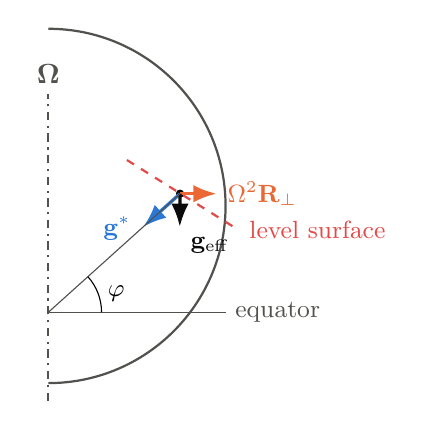
\begin{tikzpicture}[scale=0.75]
  \def\R{3.0}
  \draw[thick,cMuted] (0,-1.2) arc[start angle=-90,end angle=90,radius=\R] ;
  \draw[thick,cMuted,dash dot] (0,-1.5) -- (0,3.7) node[above] {$\bm\Omega$};
  \draw[cMuted] (0,0) -- (\R,0) node[right] {\small equator};
  \coordinate (P) at ({\R*cos(42)},{\R*sin(42)});
  \coordinate (O) at (0,0);
  \fill (P) circle (2pt);
  \draw[-{Latex},very thick,cBlue] (P) -- ($(P)!0.28!(O)$) node[pos=1.05,left,font=\small] {$\mathbf g^*$};
  \draw[-{Latex},very thick,cOrange] (P) -- ($(P)+(0.62,0)$) node[right,font=\small] {$\Omega^2\mathbf R_\perp$};
  \coordinate (G) at ($(P)!0.28!(O)+(0.62,0)$);
  \draw[-{Latex},very thick,cInk] (P) -- (G) node[below right,font=\small] {$\mathbf g_{\rm eff}$};
  \draw[dashed,cRed,thick] ($(P)+(-0.9,0.57)$) -- ($(P)+(1.0,-0.62)$) node[right,font=\small,cRed] {level surface};
  \draw[cMuted] (O) -- (P);
  \draw (0.9,0) arc[start angle=0,end angle=42,radius=0.9] node[midway,right,font=\small] {$\varphi$};
\end{tikzpicture}
\end{center}

\begin{center}
\begin{tabular}{@{}lll@{}}
\toprule
 & vertical & horizontal\\
\midrule
centrifugal $\Omega^2a\cos\varphi$ & $\Omega^2a\cos^2\varphi$ (outward) & $\Omega^2a\sin\varphi\cos\varphi$ (equatorward)\\
at the equator & $\Omega^2a=\SI{0.034}{\metre\per\second\squared}=g/290$ & 0\\
Coriolis, eastward $u$ & $2\Omega u\cos\varphi$ (up) & $2\Omega u\sin\varphi$ (equatorward)\\
\bottomrule
\end{tabular}
\end{center}

\begin{derivbox}[Coriolis from angular momentum (north--south motion)]
$A=\Omega a^2\cos^2\varphi+ua\cos\varphi$ conserved, $v=a\dot\varphi$:\quad
$\dfrac{\DD u}{\DD t}=2\Omega\sin\varphi\,v+\dfrac{uv\tan\varphi}{a}$.\quad
Ring of air from the equator: $u(\varphi)=\Omega a\,\dfrac{\sin^2\varphi}{\cos\varphi}$: $14,\,58,\,134\ \si{\metre\per\second}$ at $10^\circ,20^\circ,30^\circ$.
\end{derivbox}

\section*{3. Rules to remember}
\begin{itemize}[leftmargin=*,itemsep=1pt]
\item Coriolis: velocity-dependent, $\perp$ to motion, \emph{to the right} in the Northern Hemisphere, does no work.
\item Centrifugal: position-dependent, along $\mathbf R_\perp$, absorbed into $\mathbf g_{\rm eff}$, which defines ``down'' and the oblate shape.
\item Eastward motion $\Rightarrow$ stronger centrifugal $\Rightarrow$ equatorward drift; westward $\Rightarrow$ poleward drift; both are to the right.
\item $f=2\Omega\sin\varphi$: $\approx 0$ at the equator, \SI{1.03e-4}{\per\second} at $45^\circ$.
\end{itemize}

\begin{extrabox}[Homogeneous-Earth flattening]
Maclaurin: $f\simeq\tfrac54\,\Omega^2a/g=1/231$ (\SI{27.6}{km}) vs actual $1/298$ (\SI{21.4}{km}): dense core (Clairaut). WGS84 $g$: \SI{9.7803}{\metre\per\second\squared} (equator), \SI{9.8322}{\metre\per\second\squared} (pole); centrifugal explains $65\%$.
\end{extrabox}

\begin{verifybox}[``poleward'' effective gravity]
Slides 9--11 call the horizontal part of effective gravity \emph{poleward}. Relative to a \emph{sphere}, $\mathbf g^*+\Omega^2\mathbf R_\perp$ has an \emph{equatorward} horizontal part; relative to the \emph{bulged} surface it is gravity's own along-surface part that is poleward and balances it. Same final balance: no net horizontal force on a body at rest.
\end{verifybox}

\section*{4. Book extras (Marshall \& Plumb \S6.6) and beyond}
\begin{itemize}[leftmargin=*,itemsep=1pt]
\item Modified potential $\phi=gz-\tfrac12\Omega^2r^2$: $\ \DD\vect u/\DD t+\rho^{-1}\nabla p+\nabla\phi=-2\bm\Omega\times\vect u+\vect F$.
\item Solid-body rotation: $p/\rho+\phi=\text{const}\ \Rightarrow\ \boxed{z=h(0)+\Omega^2r^2/2g}$ (paraboloid; \SI{20}{rpm}, $r=\SI{0.5}{m}$: \SI{5.6}{cm}).
\item Radial inflow: $V_\theta r=\Omega r_1^2\Rightarrow v_\theta=\Omega(r_1^2-r^2)/r$; Rossby number $\mathrm{Ro}=U/fL\approx0.1$ at synoptic scale.
\item Eötvös: eastward $u$ changes weight by $2\Omega u\cos\varphi+u^2/a$ (\SI{30}{\metre\per\second}: $0.046\%$). Foucault: plane turns at $\Omega\sin\varphi$ (Pune \SI{75.4}{h}). Inertial oscillation: radius $U/f$, period $2\pi/f$ (\SI{10}{\metre\per\second}, $45^\circ$: \SI{97}{km}, \SI{16.9}{h}).
\end{itemize}
\end{document}
